% Options for packages loaded elsewhere
\PassOptionsToPackage{unicode}{hyperref}
\PassOptionsToPackage{hyphens}{url}
\PassOptionsToPackage{dvipsnames,svgnames,x11names}{xcolor}
%
\documentclass[
  letterpaper,
  DIV=11,
  numbers=noendperiod]{scrartcl}

\usepackage{amsmath,amssymb}
\usepackage{iftex}
\ifPDFTeX
  \usepackage[T1]{fontenc}
  \usepackage[utf8]{inputenc}
  \usepackage{textcomp} % provide euro and other symbols
\else % if luatex or xetex
  \usepackage{unicode-math}
  \defaultfontfeatures{Scale=MatchLowercase}
  \defaultfontfeatures[\rmfamily]{Ligatures=TeX,Scale=1}
\fi
\usepackage{lmodern}
\ifPDFTeX\else  
    % xetex/luatex font selection
\fi
% Use upquote if available, for straight quotes in verbatim environments
\IfFileExists{upquote.sty}{\usepackage{upquote}}{}
\IfFileExists{microtype.sty}{% use microtype if available
  \usepackage[]{microtype}
  \UseMicrotypeSet[protrusion]{basicmath} % disable protrusion for tt fonts
}{}
\makeatletter
\@ifundefined{KOMAClassName}{% if non-KOMA class
  \IfFileExists{parskip.sty}{%
    \usepackage{parskip}
  }{% else
    \setlength{\parindent}{0pt}
    \setlength{\parskip}{6pt plus 2pt minus 1pt}}
}{% if KOMA class
  \KOMAoptions{parskip=half}}
\makeatother
\usepackage{xcolor}
\setlength{\emergencystretch}{3em} % prevent overfull lines
\setcounter{secnumdepth}{5}
% Make \paragraph and \subparagraph free-standing
\makeatletter
\ifx\paragraph\undefined\else
  \let\oldparagraph\paragraph
  \renewcommand{\paragraph}{
    \@ifstar
      \xxxParagraphStar
      \xxxParagraphNoStar
  }
  \newcommand{\xxxParagraphStar}[1]{\oldparagraph*{#1}\mbox{}}
  \newcommand{\xxxParagraphNoStar}[1]{\oldparagraph{#1}\mbox{}}
\fi
\ifx\subparagraph\undefined\else
  \let\oldsubparagraph\subparagraph
  \renewcommand{\subparagraph}{
    \@ifstar
      \xxxSubParagraphStar
      \xxxSubParagraphNoStar
  }
  \newcommand{\xxxSubParagraphStar}[1]{\oldsubparagraph*{#1}\mbox{}}
  \newcommand{\xxxSubParagraphNoStar}[1]{\oldsubparagraph{#1}\mbox{}}
\fi
\makeatother


\providecommand{\tightlist}{%
  \setlength{\itemsep}{0pt}\setlength{\parskip}{0pt}}\usepackage{longtable,booktabs,array}
\usepackage{calc} % for calculating minipage widths
% Correct order of tables after \paragraph or \subparagraph
\usepackage{etoolbox}
\makeatletter
\patchcmd\longtable{\par}{\if@noskipsec\mbox{}\fi\par}{}{}
\makeatother
% Allow footnotes in longtable head/foot
\IfFileExists{footnotehyper.sty}{\usepackage{footnotehyper}}{\usepackage{footnote}}
\makesavenoteenv{longtable}
\usepackage{graphicx}
\makeatletter
\newsavebox\pandoc@box
\newcommand*\pandocbounded[1]{% scales image to fit in text height/width
  \sbox\pandoc@box{#1}%
  \Gscale@div\@tempa{\textheight}{\dimexpr\ht\pandoc@box+\dp\pandoc@box\relax}%
  \Gscale@div\@tempb{\linewidth}{\wd\pandoc@box}%
  \ifdim\@tempb\p@<\@tempa\p@\let\@tempa\@tempb\fi% select the smaller of both
  \ifdim\@tempa\p@<\p@\scalebox{\@tempa}{\usebox\pandoc@box}%
  \else\usebox{\pandoc@box}%
  \fi%
}
% Set default figure placement to htbp
\def\fps@figure{htbp}
\makeatother
% definitions for citeproc citations
\NewDocumentCommand\citeproctext{}{}
\NewDocumentCommand\citeproc{mm}{%
  \begingroup\def\citeproctext{#2}\cite{#1}\endgroup}
\makeatletter
 % allow citations to break across lines
 \let\@cite@ofmt\@firstofone
 % avoid brackets around text for \cite:
 \def\@biblabel#1{}
 \def\@cite#1#2{{#1\if@tempswa , #2\fi}}
\makeatother
\newlength{\cslhangindent}
\setlength{\cslhangindent}{1.5em}
\newlength{\csllabelwidth}
\setlength{\csllabelwidth}{3em}
\newenvironment{CSLReferences}[2] % #1 hanging-indent, #2 entry-spacing
 {\begin{list}{}{%
  \setlength{\itemindent}{0pt}
  \setlength{\leftmargin}{0pt}
  \setlength{\parsep}{0pt}
  % turn on hanging indent if param 1 is 1
  \ifodd #1
   \setlength{\leftmargin}{\cslhangindent}
   \setlength{\itemindent}{-1\cslhangindent}
  \fi
  % set entry spacing
  \setlength{\itemsep}{#2\baselineskip}}}
 {\end{list}}
\usepackage{calc}
\newcommand{\CSLBlock}[1]{\hfill\break\parbox[t]{\linewidth}{\strut\ignorespaces#1\strut}}
\newcommand{\CSLLeftMargin}[1]{\parbox[t]{\csllabelwidth}{\strut#1\strut}}
\newcommand{\CSLRightInline}[1]{\parbox[t]{\linewidth - \csllabelwidth}{\strut#1\strut}}
\newcommand{\CSLIndent}[1]{\hspace{\cslhangindent}#1}

\usepackage{booktabs}
\usepackage{longtable}
\usepackage{array}
\usepackage{multirow}
\usepackage{wrapfig}
\usepackage{float}
\usepackage{colortbl}
\usepackage{pdflscape}
\usepackage{tabu}
\usepackage{threeparttable}
\usepackage{threeparttablex}
\usepackage[normalem]{ulem}
\usepackage{makecell}
\usepackage{xcolor}
\KOMAoption{captions}{tableheading}
\makeatletter
\@ifpackageloaded{caption}{}{\usepackage{caption}}
\AtBeginDocument{%
\ifdefined\contentsname
  \renewcommand*\contentsname{Table of contents}
\else
  \newcommand\contentsname{Table of contents}
\fi
\ifdefined\listfigurename
  \renewcommand*\listfigurename{List of Figures}
\else
  \newcommand\listfigurename{List of Figures}
\fi
\ifdefined\listtablename
  \renewcommand*\listtablename{List of Tables}
\else
  \newcommand\listtablename{List of Tables}
\fi
\ifdefined\figurename
  \renewcommand*\figurename{Figure}
\else
  \newcommand\figurename{Figure}
\fi
\ifdefined\tablename
  \renewcommand*\tablename{Table}
\else
  \newcommand\tablename{Table}
\fi
}
\@ifpackageloaded{float}{}{\usepackage{float}}
\floatstyle{ruled}
\@ifundefined{c@chapter}{\newfloat{codelisting}{h}{lop}}{\newfloat{codelisting}{h}{lop}[chapter]}
\floatname{codelisting}{Listing}
\newcommand*\listoflistings{\listof{codelisting}{List of Listings}}
\makeatother
\makeatletter
\makeatother
\makeatletter
\@ifpackageloaded{caption}{}{\usepackage{caption}}
\@ifpackageloaded{subcaption}{}{\usepackage{subcaption}}
\makeatother

\usepackage{bookmark}

\IfFileExists{xurl.sty}{\usepackage{xurl}}{} % add URL line breaks if available
\urlstyle{same} % disable monospaced font for URLs
\hypersetup{
  pdftitle={Detecting misfitting items in Rasch models},
  pdfauthor={Magnus Johansson},
  pdfkeywords={Rasch, Psychometrics, Item fit, Simulation},
  colorlinks=true,
  linkcolor={blue},
  filecolor={Maroon},
  citecolor={Blue},
  urlcolor={Blue},
  pdfcreator={LaTeX via pandoc}}


\title{Detecting misfitting items in Rasch models}
\author{Magnus Johansson}
\date{2025-01-03}

\begin{document}
\maketitle
\begin{abstract}
Psychometrics in general have long relied on rule-of-thumb cutoff values
for various goodness of fit metrics. With more powerful personal
computers it is both feasible and desirable to use simulation/bootstrap
methods to determine appropriate cutoff values. This paper illustrates
and evaluates the use of an R package for Rasch psychometrics that has
implemented functions to simplify the process of identifying misfitting
items using simulation based cutoff values. Through a series of
simulation studies a comparison is made between information weighted
conditional item fit and item-restscore using Goodman and Kruskal's
gamma.
\end{abstract}


\section{Introduction}\label{introduction}

This paper presents a series of simulations conducted to evaluate
methods to detect of item misfit in Rasch models. First, conditional
item infit and outfit will be under scrutiny. Second, item infit will be
compared to item-restscore (Kreiner 2011; Mueller and Santiago 2022).
Third, a bootstrap method for item-restscore will be presented and
tested.

Müller (2020) showed how the range of critical values for conditional
item infit varies with sample size. The expected average item
conditional infit range was described by Müller as fairly well captured
by Smith's rule-of-thumb formula 1±2/√n (Smith, Schumacker, and Bush
1998). However, the average range does not apply for all items, since
item location also affects model expected item fit which means that some
items may have plausible item fit values outside Smith's average value
range.

It is here proposed that by using parametric bootstrapping one can
establish item fit critical cutoff values that are sample and item
specific. The R package \texttt{easyRasch} (Johansson 2024) includes a
function to determine item infit and outfit cutoff values, which will be
tested in the simulations in this paper.

It is important to note that the conditional item fit described by
Müller (2020) and implemented in the \texttt{iarm} R package (Mueller
and Santiago 2022) should not be confused with the unconditional item
fit implemented in software such as Winsteps and RUMM2030, as well as
all R packages except \texttt{iarm}. Unconditional item fit can result
in unreliable item fit in sample sizes as small as 250 with increasing
likelihood of problems as sample size increases. Readers are strongly
recommended to read Müller's paper to fully understand the problems with
unconditional item fit.

\section{Methods}\label{methods}

\textsubscript{Source:
\href{https://pgmj.github.io/rasch_itemfit/index.qmd.html}{Article
Notebook}}

A fully reproducible manuscript with R code and data is available

The simulation of response data used three steps: first, a vector of
theta values (person scores on the latent variable) were generated using
\texttt{rnorm(mean\ =\ 0,\ sd\ =\ 1.5)}. Second, a set of item locations
ranging from -2 to 2 logits were generated for dichotomous items, using
\texttt{runif(n\ =\ 20,\ min\ =\ -2,\ max\ =\ 2)}. Third, the theta
values were used to simulate item responses for participants, using
\texttt{sim.xdim()} from the \texttt{eRm} package (Mair and Hatzinger
2007), which allows simulation of multidimensional response data.
Multiple datasets were generated using the same item and person
parameters, varying the targeting and number of the misfitting item(s).
More details are described under the separate studies below.

The parametric bootstrapping procedure was implemented using random
samples from the 10 000 simulated responses. The sample size variations
tested are described under each study.

\begin{enumerate}
\def\labelenumi{\arabic{enumi}.}
\tightlist
\item
  Estimation of item locations based on simulated item responses using
  conditional maximum likelihood (CML, Mair and Hatzinger 2007).
\item
  Estimation of sample theta values using weighted maximum likelihood
  (Warm 1989)
\item
  Simulation of new response data, fitting the Rasch model, using the
  estimated item locations and theta values.
\item
  Estimation of the dichotomous Rasch model for the new response data
  using CML.
\item
  Based on step 4, calculation of conditional item fit (Müller 2020;
  Mueller and Santiago 2022) and/or item-restscore metrics (Kreiner
  2011; Mueller and Santiago 2022).
\end{enumerate}

Steps three and four were iterated over, using resampling with
replacement from the estimated theta values as a basis for simulating
the response data in step three.

Summary statistics were created with focus on the percentage of correct
detection of misfit and false positives.

\textsubscript{Source:
\href{https://pgmj.github.io/rasch_itemfit/index.qmd.html}{Article
Notebook}}

\textsubscript{Source:
\href{https://pgmj.github.io/rasch_itemfit/index.qmd.html}{Article
Notebook}}

\textsubscript{Source:
\href{https://pgmj.github.io/rasch_itemfit/index.qmd.html}{Article
Notebook}}

\section{Study 1}\label{study-1}

Item mean square standardized residuals are either unweighted, which is
referred to as ``outfit'', or information weighted, which we call
``infit'' (Ostini and Nering 2006, 86--87). For details on conditional
item fit we refer to the previously mentioned paper by Müller (2020).

Main lines of inquiry:

\begin{enumerate}
\def\labelenumi{\arabic{enumi}.}
\tightlist
\item
  How does the number of iterations used in RIgetfit() impact the
  indicated cutoff values?
\item
  How useful are the cutoff values in detecting misfitting items (and
  false positives), when using the optimal number of iterations?
\item
  Müller (2020) hints at outfit being less useful than infit. We will
  investigate this by comparing them.
\end{enumerate}

20 dichotomous items are used, with one item misfitting. Item locations
are the same throughout. The location of the misfitting item relative
the to the sample theta mean was selected to be approximately 0, -1, and
-2 logits. Three separate datasets were generated with these variations,
each with 10 000 simulated respondents. One dataset with all three
misfitting items was also generated, using the same sample size.

The function \texttt{RIgetfit()} from the \texttt{easyRasch} R package
is tested here. It's source code can be accessed on GitHub. The function
offers the user a choice of the number of bootstrap iterations to use to
calculate the cutoff values for infit and outfit.

Then the \texttt{RIitemfit()} function is used to summarize the
bootstrap results and also calculates the infit and outfit for each item
in the observed data and highlights items with infit/outfit values
outside of the cutoff values. \texttt{RIitemfit()} has a default (user
modifiable) setting to slightly truncate the distribution of values
using \texttt{stats::quantile()} at 0.001 and 0.999 to remove extreme
values. An example is demonstrated in Table~\ref{tbl-itemfit1}, using a
subset of the items used in the simulations. Figure~\ref{fig-itemfit1}
provides a visualization of the distribution of bootstrapped infit and
outfit values, together with the infit/outfit values from the observed
data illustrated using an orange diamond shape. Note the variation
between items in plausible values of infit and outfit based on the
bootstrap, and that Smith's rule-of-thumb regarding infit (1±2/√n) would
be 0.9-1.1 for a sample size of 400.

This study was rather computationally demanding since each simulation
run entailed 100-400 underlying simulations. The sample sizes used were
150, 250, 500, and 1000. The number of iterations to determine cutoff
values were 100, 200, and 400. Sample size and iteration conditions were
fully crossed with each other and the three different targeting
variations of the one misfitting item, resulting in 4\emph{3}3 = 36
conditions. Each combination used 200 simulation runs. The simulations
took about 12 hours to run on a Macbook Pro Max M1 using 9 CPU cores.

\begin{longtable}[]{@{}
  >{\raggedright\arraybackslash}p{(\linewidth - 14\tabcolsep) * \real{0.0549}}
  >{\raggedleft\arraybackslash}p{(\linewidth - 14\tabcolsep) * \real{0.0989}}
  >{\raggedright\arraybackslash}p{(\linewidth - 14\tabcolsep) * \real{0.1868}}
  >{\raggedleft\arraybackslash}p{(\linewidth - 14\tabcolsep) * \real{0.1099}}
  >{\raggedright\arraybackslash}p{(\linewidth - 14\tabcolsep) * \real{0.1978}}
  >{\raggedright\arraybackslash}p{(\linewidth - 14\tabcolsep) * \real{0.1209}}
  >{\raggedright\arraybackslash}p{(\linewidth - 14\tabcolsep) * \real{0.1319}}
  >{\raggedleft\arraybackslash}p{(\linewidth - 14\tabcolsep) * \real{0.0989}}@{}}

\caption{\label{tbl-itemfit1}Conditional item fit with simulation based
cutoff values}

\tabularnewline

\toprule\noalign{}
\begin{minipage}[b]{\linewidth}\raggedright
Item
\end{minipage} & \begin{minipage}[b]{\linewidth}\raggedleft
InfitMSQ
\end{minipage} & \begin{minipage}[b]{\linewidth}\raggedright
Infit thresholds
\end{minipage} & \begin{minipage}[b]{\linewidth}\raggedleft
OutfitMSQ
\end{minipage} & \begin{minipage}[b]{\linewidth}\raggedright
Outfit thresholds
\end{minipage} & \begin{minipage}[b]{\linewidth}\raggedright
Infit diff
\end{minipage} & \begin{minipage}[b]{\linewidth}\raggedright
Outfit diff
\end{minipage} & \begin{minipage}[b]{\linewidth}\raggedleft
Location
\end{minipage} \\
\midrule\noalign{}
\endhead
\bottomrule\noalign{}
\endlastfoot
V1 & 1.017 & {[}0.862, 1.162{]} & 1.061 & {[}0.647, 1.423{]} & no misfit
& no misfit & -1.37 \\
V11 & 1.000 & {[}0.839, 1.21{]} & 1.032 & {[}0.742, 1.289{]} & no misfit
& no misfit & -0.66 \\
V3 & 1.022 & {[}0.902, 1.098{]} & 1.050 & {[}0.662, 1.498{]} & no misfit
& no misfit & 0.46 \\
V12 & 0.966 & {[}0.827, 1.19{]} & 0.793 & {[}0.783, 1.306{]} & no misfit
& no misfit & 1.58 \\

\end{longtable}

\textsubscript{Source:
\href{https://pgmj.github.io/rasch_itemfit/index.qmd.html}{Article
Notebook}}

\phantomsection\label{cell-fig-itemfit1}
\begin{figure}[H]

\centering{

\pandocbounded{\includegraphics[keepaspectratio]{index_files/figure-pdf/fig-itemfit1-1.pdf}}

}

\caption{\label{fig-itemfit1}Distribution of simulation based item fit
and estimated item fit from observed data}

\end{figure}%

\textsubscript{Source:
\href{https://pgmj.github.io/rasch_itemfit/index.qmd.html}{Article
Notebook}}

\textsubscript{Source:
\href{https://pgmj.github.io/rasch_itemfit/index.qmd.html}{Article
Notebook}}

\textsubscript{Source:
\href{https://pgmj.github.io/rasch_itemfit/index.qmd.html}{Article
Notebook}}

\subsection{Results}\label{results}

\textsubscript{Source:
\href{https://pgmj.github.io/rasch_itemfit/index.qmd.html}{Article
Notebook}}

Figures show the percent of simulation runs that have identified an item
as misfitting. Items with more than 5\% are colored in light red. A
number representing the detection rate is shown adjacent to the bar
representing the misfitting item. The figure grid columns are labelled
with the number of iterations used by \texttt{RIgetfit()} to determine
cutoff values, and grid rows are labelled with the sample size.

\subsubsection{Infit}\label{infit}

\phantomsection\label{cell-fig-ifb0}
\begin{figure}[H]

\centering{

\pandocbounded{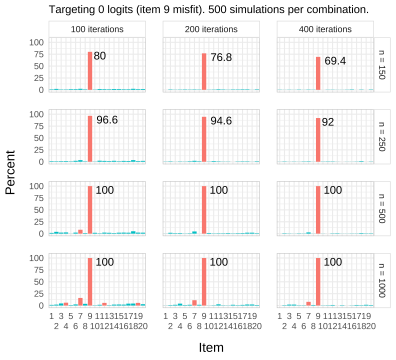
\includegraphics[keepaspectratio]{index_files/figure-pdf/fig-ifb0-1.pdf}}

}

\caption{\label{fig-ifb0}}

\end{figure}%

\textsubscript{Source:
\href{https://pgmj.github.io/rasch_itemfit/index.qmd.html}{Article
Notebook}}

Figure~\ref{fig-ifb0} shows the detection rate when the misfitting item
is located at the sample mean. Detection rate is highest for the
condition with 100 iterations with sample size 100 and 250, but it also
shows higher levels of false positives when sample size increases to 500
or more.

\phantomsection\label{cell-fig-ifb1}
\begin{figure}[H]

\centering{

\pandocbounded{\includegraphics[keepaspectratio]{index_files/figure-pdf/fig-ifb1-1.pdf}}

}

\caption{\label{fig-ifb1}}

\end{figure}%

\textsubscript{Source:
\href{https://pgmj.github.io/rasch_itemfit/index.qmd.html}{Article
Notebook}}

When the misfitting item is offset in targeting by -1 logits compared to
the sample mean (see Figure~\ref{fig-ifb1}), the smallest sample size
has less power to detect misfit compared to the on-target misfitting
item. There are lower rates of false positives across all sample sizes
and iterations.

\phantomsection\label{cell-fig-ifb2}
\begin{figure}[H]

\centering{

\pandocbounded{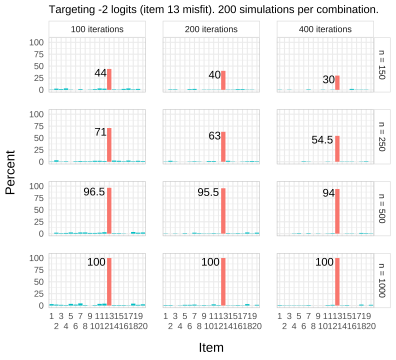
\includegraphics[keepaspectratio]{index_files/figure-pdf/fig-ifb2-1.pdf}}

}

\caption{\label{fig-ifb2}}

\end{figure}%

\textsubscript{Source:
\href{https://pgmj.github.io/rasch_itemfit/index.qmd.html}{Article
Notebook}}

Finally, when the misfitting item is located at -2 logits compared to
the sample mean (see Figure~\ref{fig-ifb2}), we see a stronger reduction
in power for sample sizes 150 and 250. No false positives are
identified.

\subsubsection{Outfit}\label{outfit}

\phantomsection\label{cell-fig-ifb0out}
\begin{figure}[H]

\centering{

\pandocbounded{\includegraphics[keepaspectratio]{index_files/figure-pdf/fig-ifb0out-1.pdf}}

}

\caption{\label{fig-ifb0out}}

\end{figure}%

\textsubscript{Source:
\href{https://pgmj.github.io/rasch_itemfit/index.qmd.html}{Article
Notebook}}

\phantomsection\label{cell-fig-ifb1out}
\begin{figure}[H]

\centering{

\pandocbounded{\includegraphics[keepaspectratio]{index_files/figure-pdf/fig-ifb1out-1.pdf}}

}

\caption{\label{fig-ifb1out}}

\end{figure}%

\textsubscript{Source:
\href{https://pgmj.github.io/rasch_itemfit/index.qmd.html}{Article
Notebook}}

\phantomsection\label{cell-fig-ifb2out}
\begin{figure}[H]

\centering{

\pandocbounded{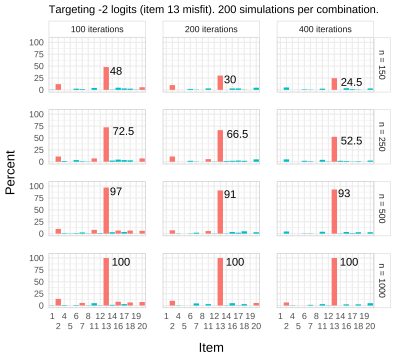
\includegraphics[keepaspectratio]{index_files/figure-pdf/fig-ifb2out-1.pdf}}

}

\caption{\label{fig-ifb2out}}

\end{figure}%

\textsubscript{Source:
\href{https://pgmj.github.io/rasch_itemfit/index.qmd.html}{Article
Notebook}}

As shown in Figure~\ref{fig-ifb0out}, Figure~\ref{fig-ifb1out}, and
Figure~\ref{fig-ifb2out}, outfit is performing much worse than infit
across the board.

\subsubsection{Comments}\label{comments}

Based on these simulation, it seems reasonable to recommend the use of
infit in determining item fit over outfit. The performance of outfit
calls to question whether it is useful at all.

Regarding infit and the use of parametric bootstrapping with
\texttt{RIgetfit()}, it looks like 100 iterations are to recommend to
determine cutoff values when the sample size is 250 or lower, while 200
or 400 iterations reduce the risk for false positives at sample sizes of
500 or larger. False positives are found at sample sizes 500 and 1000
only. The risk for false positives is notably higher when the misfitting
item is located at the sample mean compared to when the misfitting item
is off-target by -1 logits or more.

\section{Study 2}\label{study-2}

\textsubscript{Source:
\href{https://pgmj.github.io/rasch_itemfit/index.qmd.html}{Article
Notebook}}

\textsubscript{Source:
\href{https://pgmj.github.io/rasch_itemfit/index.qmd.html}{Article
Notebook}}

\subsection{Results}\label{results-1}

\phantomsection\label{cell-fig-itemrestscore1}
\begin{figure}[H]

\centering{

\pandocbounded{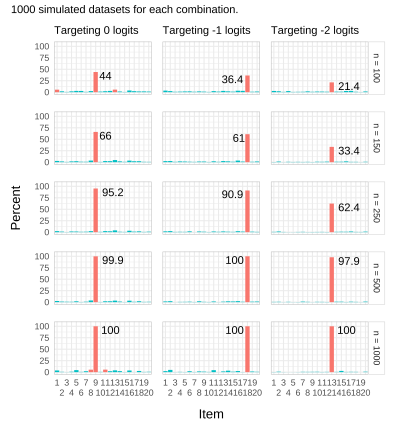
\includegraphics[keepaspectratio]{index_files/figure-pdf/fig-itemrestscore1-1.pdf}}

}

\caption{\label{fig-itemrestscore1}}

\end{figure}%

\textsubscript{Source:
\href{https://pgmj.github.io/rasch_itemfit/index.qmd.html}{Article
Notebook}}

This simulation includes an additional condition with 100 respondents,
which results in significantly lower detection rates than with 150
respondents. Compared to infit at 250 respondents, item-restscore has
detection rates of 95.2\%, 90.9\%, and 62.4\% for targeting 0, -1, and
-2, while infit has 96.5\%, 96.5\%, and 71\%. For sample size 500 and
1000, performance is similar, including the increased tendency for false
positives at n = 1000.

Similarly to infit, item-restscore has decreased detection rate for
off-target misfitting items. The false positive rate is lower for
item-restscore than infit for sample sizes below 1000.

\section{Study 3}\label{study-3}

We will now compare the performance of infit and item-restscore when all
three items are misfitting at the same time. This simulation will also
include a condition with 2000 respondents, to examine if the false
positive rate increases with more respondents. For infit, we will only
use 200 iterations with \texttt{RIgetfit()} since that condition seemed
to strike a balance between detection rate and false positives.

\textsubscript{Source:
\href{https://pgmj.github.io/rasch_itemfit/index.qmd.html}{Article
Notebook}}

\textsubscript{Source:
\href{https://pgmj.github.io/rasch_itemfit/index.qmd.html}{Article
Notebook}}

\textsubscript{Source:
\href{https://pgmj.github.io/rasch_itemfit/index.qmd.html}{Article
Notebook}}

\subsubsection{Results}\label{results-2}

\phantomsection\label{cell-fig-ifb3}
\begin{figure}[H]

\centering{

\pandocbounded{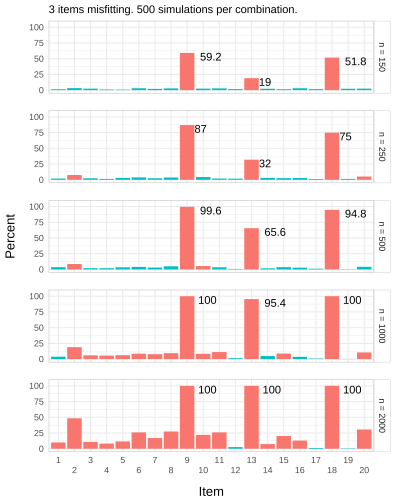
\includegraphics[keepaspectratio]{index_files/figure-pdf/fig-ifb3-1.pdf}}

}

\caption{\label{fig-ifb3}}

\end{figure}%

\textsubscript{Source:
\href{https://pgmj.github.io/rasch_itemfit/index.qmd.html}{Article
Notebook}}

\phantomsection\label{cell-fig-ifb3out}
\begin{figure}[H]

\centering{

\pandocbounded{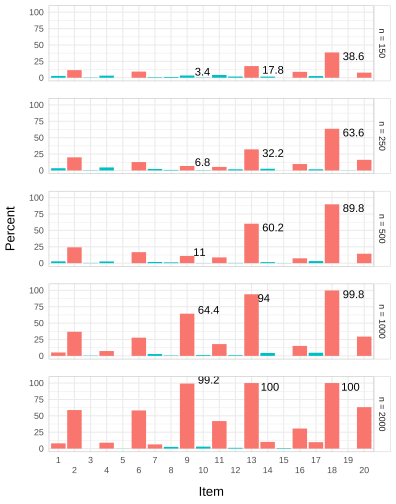
\includegraphics[keepaspectratio]{index_files/figure-pdf/fig-ifb3out-1.pdf}}

}

\caption{\label{fig-ifb3out}}

\end{figure}%

\textsubscript{Source:
\href{https://pgmj.github.io/rasch_itemfit/index.qmd.html}{Article
Notebook}}

Looking at the performance of infit with three misfitting items
(Figure~\ref{fig-ifb3}), we can see that the detection rate is markedly
worse for item 13 in sample sizes 500 and below, compared to when single
items were misfitting. The false positive rate has increased for sample
size of 1000, and we can see this escalate strongly for n = 2000. Outfit
(Figure~\ref{fig-ifb3out}) again performs worse than infit.

\phantomsection\label{cell-fig-itemrestscore2}
\begin{figure}[H]

\centering{

\pandocbounded{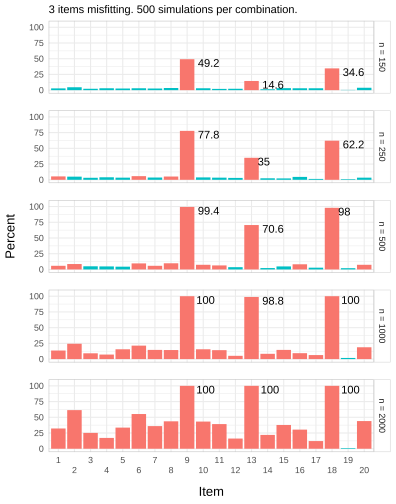
\includegraphics[keepaspectratio]{index_files/figure-pdf/fig-itemrestscore2-1.pdf}}

}

\caption{\label{fig-itemrestscore2}}

\end{figure}%

\textsubscript{Source:
\href{https://pgmj.github.io/rasch_itemfit/index.qmd.html}{Article
Notebook}}

Item-restscore has higher detection rate than infit (see
Figure~\ref{fig-itemrestscore2}), but also higher levels of false
positives.

\section{Study 4}\label{study-4}

For our final set of simulations, we will use a non-parametric bootstrap
procedure with item-restscore. First, based on the above problematic
sample size of 2000, we let the bootstrap function sample with
replacement using n = 800. 250 bootstrap samples will be used, then we
summarize the percentage indicating misfit for each item. Second, we
will also apply this to samplesizes 150, 250, and 500, and use the
complete sample for the same bootstrap procedure to see if this produces
more useful information for identifying misfitting items.

\section{Discussion}\label{discussion}

\section{Conclusion}\label{conclusion}

These findings make a good argument for removing one item at a time when
the analysis indicates misfitting items, starting with the most
misfitting item. This is especially relevant for sample sizes at 500 or
above and when misfitting items are located close to the sample mean.

\section*{References}\label{references}
\addcontentsline{toc}{section}{References}

\phantomsection\label{refs}
\begin{CSLReferences}{1}{0}
\bibitem[\citeproctext]{ref-easyrasch}
Johansson, Magnus. 2024. \emph{easyRasch: Psychometric Analysis in r
with Rasch Measurement Theory}. \url{https://github.com/pgmj/easyRasch}.

\bibitem[\citeproctext]{ref-kreiner_note_2011}
Kreiner, Svend. 2011. {``A {Note} on {Item}--{Restscore} {Association}
in {Rasch} {Models}.''} \emph{Applied Psychological Measurement} 35 (7):
557--61. \url{https://doi.org/10.1177/0146621611410227}.

\bibitem[\citeproctext]{ref-mair_extended_2007}
Mair, Patrick, and Reinhold Hatzinger. 2007. {``Extended {Rasch}
{Modeling}: {The} {eRm} {Package} for the {Application} of {IRT}
{Models} in {R}.''} \emph{Journal of Statistical Software} 20 (1):
1--20. \url{https://doi.org/10.18637/jss.v020.i09}.

\bibitem[\citeproctext]{ref-mueller_iarm_2022}
Mueller, Marianne, and Pedro Henrique Ribeiro Santiago. 2022. {``Iarm:
{Item} {Analysis} in {Rasch} {Models}.''}
\url{https://cran.r-project.org/web/packages/iarm/index.html}.

\bibitem[\citeproctext]{ref-muller_item_2020}
Müller, Marianne. 2020. {``Item Fit Statistics for {Rasch} Analysis: Can
We Trust Them?''} \emph{Journal of Statistical Distributions and
Applications} 7 (1): 5.
\url{https://doi.org/10.1186/s40488-020-00108-7}.

\bibitem[\citeproctext]{ref-ostini_polytomous_2006}
Ostini, Remo, and Michael Nering. 2006. \emph{Polytomous {Item}
{Response} {Theory} {Models}}. SAGE Publications, Inc.
\url{https://doi.org/10.4135/9781412985413}.

\bibitem[\citeproctext]{ref-smith_using_1998}
Smith, R. M., R. E. Schumacker, and M. J. Bush. 1998.
{``\href{https://www.ncbi.nlm.nih.gov/pubmed/9661732}{Using Item Mean
Squares to Evaluate Fit to the {Rasch} Model}.''} \emph{Journal of
Outcome Measurement} 2 (1): 66--78.

\bibitem[\citeproctext]{ref-warm_weighted_1989}
Warm, Thomas A. 1989. {``Weighted Likelihood Estimation of Ability in
Item Response Theory.''} \emph{Psychometrika} 54 (3): 427--50.
\url{https://doi.org/10.1007/BF02294627}.

\end{CSLReferences}




\end{document}
